% --------------------------------------------------------------
% This is all preamble stuff that you don't have to worry about.
% Head down to where it says "Start here"
% --------------------------------------------------------------

\documentclass[11pt]{scrartcl}

\usepackage{natbib}
\usepackage{geometry}
\usepackage{amsmath,amsthm,amssymb,url}
\usepackage{fullpage}
\usepackage{tabularx}
\usepackage{float}
\usepackage{microtype}
\usepackage[pdftex]{hyperref}

\usepackage[final]{graphicx}
\usepackage{xcolor}
\definecolor{darkblue}{rgb}{0,0,0.5}
\usepackage{transparent}

\usepackage{enumitem}
\setlist{nolistsep}

\setlength{\parskip}{3px}

%\addtolength{\topmargin}{-.5in}
%\addtolength{\textheight}{1.2in}

\newcommand{\N}{\mathbb{N}}
\newcommand{\Z}{\mathbb{Z}}

\newenvironment{theorem}[2][Theorem]{\begin{trivlist}
\item[\hskip \labelsep {\bfseries #1}\hskip \labelsep {\bfseries #2.}]}{\end{trivlist}}
\newenvironment{lemma}[2][Lemma]{\begin{trivlist}
\item[\hskip \labelsep {\bfseries #1}\hskip \labelsep {\bfseries #2.}]}{\end{trivlist}}
\newenvironment{exercise}[2][Exercise]{\begin{trivlist}
\item[\hskip \labelsep {\bfseries #1}\hskip \labelsep {\bfseries #2.}]}{\end{trivlist}}
\newenvironment{problem}[2][Problem]{\begin{trivlist}
\item[\hskip \labelsep {\bfseries #1}\hskip \labelsep {\bfseries #2.}]}{\end{trivlist}}
\newenvironment{question}[2][Question]{\begin{trivlist}
\item[\hskip \labelsep {\bfseries #1}\hskip \labelsep {\bfseries #2.}]}{\end{trivlist}}
\newenvironment{corollary}[2][Corollary]{\begin{trivlist}
\item[\hskip \labelsep {\bfseries #1}\hskip \labelsep {\bfseries #2.}]}{\end{trivlist}}

\begin{document}

% --------------------------------------------------------------
%                         Start here
% --------------------------------------------------------------

\title{Visualizing Physical Query Execution in a Relational Distributed Big Data Management System}
\subtitle{Project Description \--- Distributed Systems}
\author{Shumo Chu and Dominik Moritz}
\date{}

\maketitle

\section{Introduction}

Myria is a distributed big data management system currently being developed in the database group. Myria aims towards building a distributed database platform to provide \emph{big data management and analytics as a service} primarily for scientific applications. Myria can run queries from languages that are equivalent to relational algebra with recursion. Queries are translated to physical query execution plans and then executed in the system. At the moment, the only measure for query execution is the overall running time. This limitation led to extended debugging sessions where we tried to understand why certain queries run for a long time. This process was often not very successful and is clearly not effective as understanding system behavior in a distributed database management system requires observing related executions across different workers.

We are building a system to collect information about the query execution and visualize the data in a meaningful way that will allow us to efficiently debug and improve query execution. An example of our visualization can be seen in Figure~\ref{fig:fig1}.

\begin{figure}[H]
  \begin{center}
    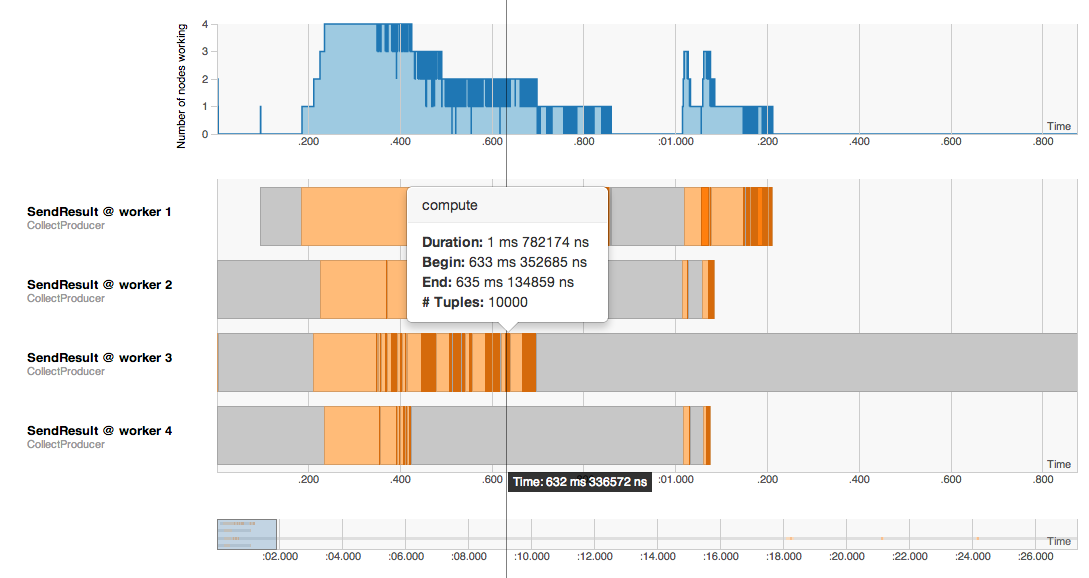
\includegraphics[width=.8\textwidth]{figure1}
  \end{center}
  \caption{Visualization of fragment execution and worker utilization with focus on the first two seconds.}
  \label{fig:fig1}
\end{figure}


\section{Background and goals}

This section describes how queries are executed in the Myria system and how our project will help us to understand the execution of physical query plans.


\subsection{Background}
\label{sec:background}

The Myria database system needs to transform user's high-level queries, eg. SQL, Datalog, or Myrial\footnote{Myrial is a PigLatin like declarative language} into a physical query plan. The physical query plan is the actual execution map. Usually it can be viewed as a \emph{DAG}, which consists of basic operators, such as \emph{JOIN}, \emph{GROUP BY}, \emph{SCAN}, \emph{APPLY} and relational tables. In distributed database systems, the introduction of the \emph{SHUFFLE} operator and data partitioning makes query plans more complicated.

\begin{figure}
 \begin{center}
     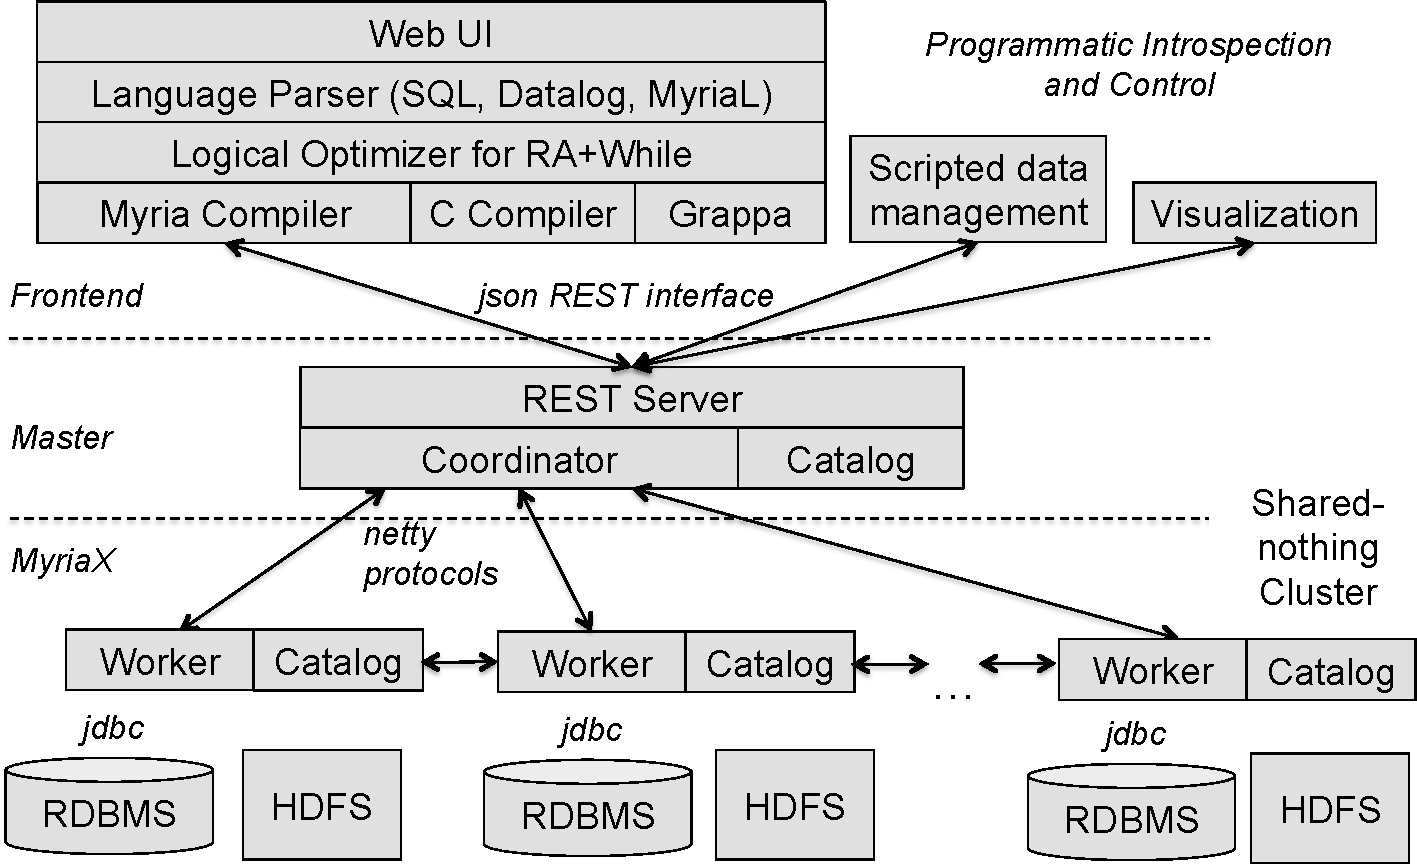
\includegraphics[width=0.7\textwidth]{arch}
   \end{center}
  \caption{Myria System Architecture.}
  \label{fig:myria_arc}
\end{figure}

Figure~\ref{fig:myria_arc} shows the overall system architecture consisting of the front-end and the Myria database consisting of the master and the distributed execution engine. The center component in Figure~\ref{fig:myria_arc} is the master. It hosts the REST interface used by the web UI and other tools, maintains metadata about the system resources and datasets in the cluster (e.g., used by the query optimizer in the web UI), and it mediates access to the cluster itself. Database queries in the form of SQL, Myrial, or Datalog are translated to the physical query plan.

The bottom part shows the architecture of Myria’s query execution engine, MyriaX. MyriaX is a pipelined, parallel, distributed dataflow evaluation system that takes a (possibly cyclic) graph of operators (query plan) and executes it efficiently on a shared-nothing cluster. This pipeline is divided into query fragments, which are chains of operators that can operate on a single compute node in a single thread. The data is pre-partitioned and stored in the workers.

A query plan is the actual execution map for the distributed database system.  Each query plan consists of basic operators forming an execution flow. For example, the SQL query $SELECT \; R.*, S.*  \; WHERE \; R.x=S.y ;$ can be translated to the visualized query plan shown in Figure~\ref{fig:query_plan}. The semantics of the query plan is a distributed hash join of two tables, $R$ and $S$. We first need to hash each table according to the joined fields. Then tuples are shuffled by their hash results to different workers. At each worker, the shuffled tuples are joined locally. A query fragment is a subtree of the query execution plan that is separated from the rest of the plan by a network boundary. The example has three query fragments denoted by different colors.

Each query fragment runs in a separate thread on each worker and is separated from other query fragments by a network boundary. Myria's execution model is asynchronous and pull based within one fragment and push based between fragments. This means that within one query fragment an operator calls its children to fetch data. A child can either return \texttt{null} if no or not enough data is ready or a tuple batch. When a root operator in a query fragment is a shuffle producer, it shuffles tuples to other fragments. Note that the query fragments together do not necessarily form a DAG because of recursion.

\begin{figure}
 \begin{center}
     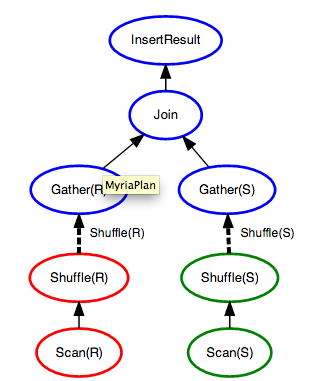
\includegraphics[width=0.35\textwidth]{partition_join.png}
   \end{center}
  \caption{Query plan: distributed hash join using three query fragments.}
  \label{fig:query_plan}
\end{figure}

The Myria database is written in Java and communicates using protocol buffers. The Myria web front end is written in python and runs on App engine.


\subsection{Goals}
\label{sec:objective}

Database system profiling has been extensively studied over decades. There are two types of works on this topic. One is logging query execution information and analyzing logs afterwards for better query optimization. The other is using real-time profiling information to estimate the progress of a query. We focus on the first type of problem in the context of distributed database system.

Our system has to collect information about the execution of a physical query plan in Myria, which provides the foundation for analyzing the data and creating a meaningful visualization. The visualization will be embedded in a web application. We plan to analyze the query execution and find problems such as data skew.

\vspace{5px}

\noindent Questions that we want to answer with this project:

\begin{enumerate}
  \item What are the data dependencies between operators in workers?
  \item What is the bottleneck of the execution? Improving which part could improve the performance the most?
    %\item How does an optimization rule affect query execution?
  %\item Is an execution network or CPU bound?
  \item Is there a slow worker during a certain stage of the execution that prevent the progress of the whole query plan?
  \item Is the data skewed in a way that prevents efficient usage of available workers?
  \item How does network and computation contribute to the total running time? We make two hypothesis, respectively. If we assume the network has infinite bandwidth and no latency, how would the running time change? If we assume that we have infinite computation power, how would the running time change?
  %\item How good is the load balancing? If it is skewed, how much does this affect the performance?

\end{enumerate}

We do not try to build a visualization that can visualize long running queries with many states for each query fragment as we do not expect to get different insights into the general query execution, skew and data flow from queries that run longer. However, since we can have many workers and multiple query fragments, which will prevent us from showing all profiling data in one view.

% explain what we want to learn about operators, query fragments and workers
% talk about shared memory model


\section{Related work}

Tools to visualize query plans for example in SQL Server as used to improve performance for the SDSS Sky survey\cite{szalay2002sdss} focus on optimizing queries and not query execution and have no visualization of data flow which is necessary to optimize physical query execution.

Twitter developed Ambrose\cite{ambrose}, a platform for visualization and real-time monitoring of MapReduce data workflows. They offer three different views to show associated jobs, job dependencies and progress. Ambrose has been released as open source. Ambrose, however, is not suitable for our needs as the abstraction level of jobs is too high and does not capture single operators.

Google's Dapper\cite{sigelman2010dapper} is a distributed systems tracing infrastructure offers more fine grained tracing of calls in their distributed system. Twitter closely modelled Zipkin\cite{zipkin} after Dapper and released it as open source. Our system is similar to Dapper and Zipkin has a similar architecture and offers similar visualizations. However, we offer different abstraction levels which enables users to find problems faster and handle larger amounts of profiling data. Also, our visualization is optimized to help developers understand query execution in Myria as opposed to general traces in distributed systems.


\section{Design and implementation}

In Section~\ref{sec:logging}, we will describe how we collect performance data using logging and what the logs tell us about the query execution. Section~\ref{sec:collect} explains how logs are collected. In Section~\ref{sec:visualization}, we will focus on how we present this information to help us as developers to understand the performance impact of skew or certain operators on the running time.

In Section~\ref{sec:overhead}, we will explain a method that we use to determine the communication and computation time of a query execution.


\subsection{Logging}
\label{sec:logging}

In our visualization, we want to capture the state of operators, query fragments, and workers. A state is similar to a span in Dapper\cite{sigelman2010dapper}.

The state of a query fragment depends on the state of the operators inside it and the state of a worker depends on the state of the query fragments that are running on it. Consequently, we only need to capture the state of query fragments per worker. In order to capture state changes, we log events and state changes of operators. In the logs we look for events that indicate a state change. For each state we want to visualize when the transitions happened.

Not all operators have the same states. A consumer for example does not have a wait, compute or send state. Table~\ref{tbl:state} shows the different states operators can be in and briefly describes their meaning. Note that sleep and wait are different. Waiting means that an operator is waiting for child operator to return from a function call and sleep means that an operator has to be woken up by new incoming data.

\begin{table}[h]
\begin{tabularx}{\textwidth}{ l|X|X|X }
 & \multicolumn{3}{ c }{operator type} \\
\cline{2-4}
state & producers (pushes to other fragments) & consumers (receive from other fragments) & operations \newline (\emph{JOIN}, \emph{MERGE}, \emph{SCAN}, \emph{APPLY}, ...) \\
\hline \hline
receive & - & receives data from producer over network & - \\
\hline
wait & child is producing & - & waiting for child to return \\
\hline
compute & hashing data & - & in \texttt{fetchNextReady} and not waiting for any data \\
\hline
sleep & has data for consumer that is not ready & no data in producer & waiting for signal \\
\hline
send & sending data to consumer over network & - & - \\
\end{tabularx}
\caption{Possible states of operators and their meaning.}
\label{tbl:state}
\end{table}

In order to capture these states we have to log events that indicate their beginning and their end. An operator can only be in one state at a time. Consequently, the states can be reconstructed from the logs without any information about which events belong to each other. Since we also log the time of the events we can reconstruct when an operator changes its state and determine how long it has been in a certain state. We don't expect clock skew to be a problem because the intervals are coarse grained enough.

No all transitions between states are possible. For example, the wait state can only be reached from the compute state. A way to interpret this is that wait and compute are a sub-states of another state work. This interpretation is useful since a set of computes and waits can be grouped together because they were triggered by a call to \texttt{fetchNextReady} and end with a return from the function. We will use this information in the visualization of operator states.

To be able to reconstruct the states mentioned in Table~\ref{tbl:state} we have to log all events that cause state changes.

As mentioned in the beginning of this section, the states of query fragments and workers can be inferred from the state of the query fragments that are executed on a worker. A query fragment can be in the state receiving when the leaf operator is a consumer (and not a scan). It can be in the state compute when any of its children are computing. It can be sleeping when the root is sleeping and it can be sending when the root is sending. Since a fragment is executed by one thread, it cannot be in multiple states.

The state of a worker is ambiguous because multiple threads can be executing multiple query fragments that are in different states. We will use the state of the query fragments to show how many query fragments are working but we will not determine a single state for the whole worker.

% state changes

\subsection{Log collection}
\label{sec:collect}

For logging, we use standard Java logging using \emph{slf4j}\footnote{\url{http://www.slf4j.org}}, a logging API, which is implemented by different logging frameworks. Since logs are collected on different workers, we need to collect them on one machine that analyzes the data and creates the visualizations. The collecting server is a Myria worker, which means that we can use its database to store the logs and then read from when we create the visualization. We have not been implemented storing the data in the database yet and read the logs in each request from the web front end.

This architecture of distributed loggers and collectors is similar to the collection pipeline proposed in Dapper\cite{sigelman2010dapper}.

Logs are collected on the Myria master that offers a REST API to access the aggregated and preprocessed data. The visualization fetches data using Ajax\footnote{Asynchronous JavaScript calls to a server.} from the Myria through the App engine server for myria web. We use this indirection to aggregate data for visualization as we want the Myria REST API to stay simple.


\subsection{Visualization}
\label{sec:visualization}

Users can switch between three levels of query execution visualization to identify the problem at the granularity that best reveals the information they need. These kinds of visualization allow developers to answer the questions from Section~\ref{sec:objective}.

% except for the last one. We will describe how we answer this question in Section~\ref{sec:overhead}.

A more detailed evaluation of how the visualization helped us to understand, debug and eventually improve how queries are executed will be given in Section~\ref{sec:evaluation}.

\subsubsection{Query plan level}

The query plan level visualization as seen in Figure~\ref{fig:frags} shows a line chart of utilization of the cluster for each query fragment. Utilization is measured as the fraction of workers that are executing the query fragment. By observing long tails users can identify which of the query fragments is a bottleneck. Skew can be identified in a drop in the number of workers calculating a query fragment.

\begin{figure}[h]
  \begin{center}
    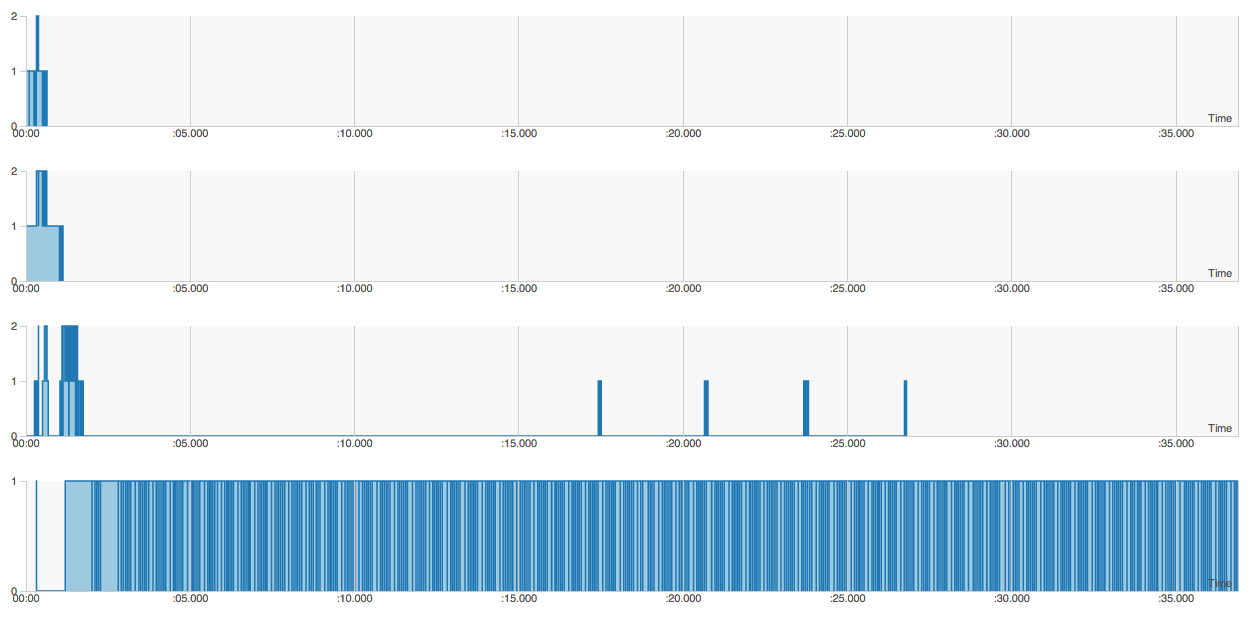
\includegraphics[width=\textwidth]{fragments_lines}
  \end{center}
  \caption{Visualization that shows on how many workers a fragment is computing. The last fragment is the one that writes the join results to disk.}
  \label{fig:frags}
\end{figure}


\subsubsection{Query fragment level}

If a critical fragment is identified, a user can switch to the visualization at the query fragment level. This level shows the execution state of the same query fragment on different workers in a Gantt chart as seen in Figure~\ref{fig:fig1}. Possible states of a fragment are \emph{computing}, \emph{waiting}, and \emph{sleeping}. Gantt charts are used widely in the visualization of project plans because they visualize time spans and show dependencies between them. The state of a fragment is defined by the state of the root operator. Users can finally narrow down to identify which worker to explore next.


\subsubsection{Operator level}

The operator level visualization as seen in Figure~\ref{fig:gantt} shows a Gantt chart of the operator states for a specific query fragment. The operators of the query fragment are shown in the same hierarchy as they appear in the query subtree. For every point in time, the Gantt chart shows the operator states, \emph{computing}, \emph{waiting} (an operator waits for a call to its child to return), \emph{sleeping}, \emph{receiving}, or \emph{sleeping}. This view allows users to see which operator is the bottleneck of the query fragment and how long/how frequent an operator is waiting for data.

For the visualization of operators we want to show the hierarchical relationship between operators and allow users to focus only on certain operators. Additional information about states (such as where the data is fetched from, specific parameters of an operator and eventually how much data was returned) will be shown on demand.

\begin{figure}[h]
  \begin{center}
    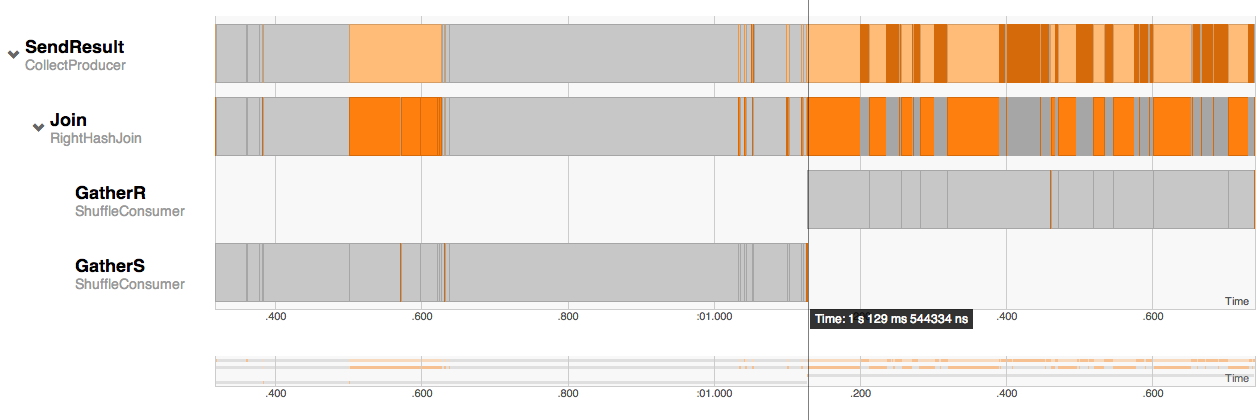
\includegraphics[width=\textwidth]{join_gantt}
  \end{center}
  \caption{Query fragment of hash join that first consumes all tuples from S and then joins with R. Orange is computing, light orange is waiting and gray is sleeping. The small graph under the main graph allows users to select an area to focus on.}
  \label{fig:gantt}
\end{figure}


% For the final visualization, we plan to add another view that shows the graph that shows on how many workers a query fragment is running for each query fragment. The three views can be seen as showing different granularities. The overview over all query fragments reveals dependencies and a developer might want to investigate a certain query fragment that seems to block others. For this query fragment the developer can investigate its execution of different workers and potentially find the one that is slowing down the whole execution. Then the developer can evaluate why a particular query fragment on a worker is not working.

\subsubsection{Implementation}

We use D3\cite{bostock2011d3} to build the visualization. D3 is a JavaScript framework for data visualizations on the web. Consequently, our visualization will be browser based and we integrated it into the existing web interface for Myria\footnote{A demo can be found at \url{http://myria-web.appspot.com} but it does not yet have the visualization.}.

We used the visualization technique of \emph{focus+context}\cite{furnas1986generalized} to allow users to zoom into a detail of the query execution without loosing the context of the whole query.

The data format for the visualizations is a custom JSON\footnote{JavaScript object notation} format with nested operators and an array of states per operator. The line charts use CSV\footnote{Comma separated values}.


\section{Evaluation}
\label{sec:evaluation}

TODO: Shumo

% talk about how we use it in demo for sigmod


\section{Outlook}
\label{sec:outlook}

In this paper, we explained Myria's execution model and our log collection and log analysis infrastructure and our visualization. We also evaluated what our current visualization offers to developers. Nonetheless, further improvements of the performance (Section~\ref{sec:performance}) and the visualization (Section~\ref{sec:vizimprovement}) are possible.

In Section~\ref{sec:overhead}, we will explain a method that we use to determine the communication and computation time of a method that we use to determine the communication and computation time of a query execution.


\subsection{Visualization and integration}
\label{sec:vizimprovement}

We plan better integration of the visualization into the web interface and automatically redirect users to the overview visualization when they submit a long running queries. The visualization can then be used to help estimating the progress of the query execution.

In addition to a better integration into the user interface, we plan to improve the Gantt chart for operator visualization to better present dependencies and explicitly show nesting. We already have some mock-ups that we created in response to what we saw in our charts but plan to first finish the back end to make it easier to adapt the data format.

Another small improvement that we plan to implement is to show how many tuples were sent to the same worker and how many tuples had to be sent to other servers.


\subsection{Performance}
\label{sec:performance}

We plan to improve the performance of the backend by storing the data in the Myria database as described in Section~\ref{sec:collect}. The performance of the front end will be improved by adapting the data schema to a format that integrates more tightly with the visualization and removes redundant information.

Even though we defined performance not be our goal in the initial design, other developers have asked us to visualize long running queries.


\subsection{Estimate computation/network overhead}
\label{sec:overhead}

A further question is  how can we get insightful information from the logging and visualization. To help us improving query plan rewriting and efficiently allocate resource for a query, we might want to reason about what factor contribute most to the running time of the query plan from the logging/visualization. In a pipelined and asynchronous query execution, since communication (via network) and computation are overlapped. There would be no accurate measure of the communication time and computation time for the whole system.  So we would like to ask following questions.

\noindent\textbf{Assume no communication time}.  That is to assume that we can have an underlying network with infinite bandwidth and zero latency. Based on the logging, we want to infer how much the running time could be improved given this assumption. This would be a measure of how expensive the computation is and could demonstrate the best performance gain we can have if we make the communication faster.

\noindent\textbf{Assume no computation time}.  That is to assume that we can have infinitely fast computation hardware. Given this assumption, we want to infer how much the running time could be improved. This would be a measure of how expensive the communication is.

\noindent\textbf{Proposed solution}.  Based on the logging information, we can build a temporal state transition graph of the query execution. This graph will consist of the temporal state information of each query fragment in each worker. Combined with the query plan which contains the dependency between different operators, we want to develop algorithms to infer the running time given different assumptions.

\bibliographystyle{plain}
\bibliography{references}

\end{document}